%
%  RULES OF THE GAME
%
%  * 80 characters
%  * line breaks at the ends of sentences
%  * eqnarrys ONLY
%  * ``light curve'' not ``light-curve'' or ``lightcurve''
%  * that is all.
%

\documentclass[12pt,preprint]{aastex}

\pdfoutput=1

\usepackage{color,hyperref}
\definecolor{linkcolor}{rgb}{0,0,0.5}
\hypersetup{colorlinks=true,linkcolor=linkcolor,citecolor=linkcolor,
            filecolor=linkcolor,urlcolor=linkcolor}
\usepackage{url}
\usepackage{amssymb,amsmath}
\usepackage{subfigure}
\usepackage{booktabs}

\newcommand{\project}[1]{\textsl{#1}} % hogg say
\newcommand{\kepler}{\project{Kepler}}
\newcommand{\KT}{\project{K2}}
\newcommand{\tess}{\project{TESS}}
\newcommand{\terra}{\project{TERRA}}
\newcommand{\license}{MIT License}
\newcommand{\projectname}{\project{ketu}}

\newcommand{\paper}{\textsl{Article}}

\newcommand{\foreign}[1]{\emph{#1}}
\newcommand{\etal}{\foreign{et\,al.}}
\newcommand{\etc}{\foreign{etc.}}
\newcommand{\True}{\foreign{True}}
\newcommand{\Truth}{\foreign{Truth}}

\newcommand{\figref}[1]{\ref{fig:#1}}
\newcommand{\Fig}[1]{Figure~\figref{#1}}
\newcommand{\fig}[1]{\Fig{#1}}
\newcommand{\figlabel}[1]{\label{fig:#1}}
\newcommand{\Tab}[1]{Table~\ref{tab:#1}}
\newcommand{\tab}[1]{\Tab{#1}}
\newcommand{\tablabel}[1]{\label{tab:#1}}
\newcommand{\Eq}[1]{Equation~(\ref{eq:#1})}
\newcommand{\eq}[1]{\Eq{#1}}
\newcommand{\eqalt}[1]{Equation~\ref{eq:#1}}
\newcommand{\eqlabel}[1]{\label{eq:#1}}
\newcommand{\Sect}[1]{Section~\ref{sect:#1}}
\newcommand{\sect}[1]{\Sect{#1}}
\newcommand{\sectalt}[1]{\ref{sect:#1}}
\newcommand{\App}[1]{Appendix~\ref{sect:#1}}
\newcommand{\app}[1]{\App{#1}}
\newcommand{\sectlabel}[1]{\label{sect:#1}}

\newcommand{\BIC}{{\ensuremath{\mathrm{BIC}}}}
\newcommand{\TIC}{{\ensuremath{\mathrm{TIC}}}}
\newcommand{\T}{\ensuremath{\mathrm{T}}}
\newcommand{\dd}{\ensuremath{\,\mathrm{d}}}
\newcommand{\bvec}[1]{{\ensuremath{\boldsymbol{#1}}}}
\newcommand{\appropto}{\mathrel{\vcenter{
  \offinterlineskip\halign{\hfil$##$\cr
    \propto\cr\noalign{\kern2pt}\sim\cr\noalign{\kern-2pt}}}}}
\newcommand{\densityunit}{{\ensuremath{\mathrm{nat}^{-2}}}}

% TO DOS
\newcommand{\todo}[3]{{\color{#2} \emph{#1} TODO: #3}}
\newcommand{\dfmtodo}[1]{\todo{DFM}{red}{#1}}
\newcommand{\hoggtodo}[1]{\todo{HOGG}{blue}{#1}}

% Notation for this paper.
\newcommand{\flux}{{\ensuremath{f}}}
\newcommand{\ferr}{{\ensuremath{\sigma_\flux}}}
\newcommand{\attime}{{\ensuremath{t}}}
\newcommand{\basis}{{\bvec{A}}}
\newcommand{\weights}{{\bvec{w}}}

\newcommand{\period}{{\ensuremath{P}}}
\newcommand{\phase}{{\ensuremath{T^0}}}
\newcommand{\duration}{{\ensuremath{D}}}
\newcommand{\depth}{{\ensuremath{Z}}}
\newcommand{\transittime}{{\ensuremath{T}}}

\begin{document}

\title{%
    A systematic search for transiting planets using \KT
}

\newcommand{\nyu}{2}
\newcommand{\caltech}{3}
\newcommand{\cfa}{4}
\newcommand{\mpia}{5}
\newcommand{\cds}{6}
\newcommand{\mpis}{7}
\author{%
    Daniel~Foreman-Mackey\altaffilmark{1,\nyu},
    Benjamin~T.~Montet\altaffilmark{\caltech,\cfa},
    David~W.~Hogg\altaffilmark{\nyu,\mpia,\cds},
    Bernhard~Sch\"olkopf\altaffilmark{\mpis},
    Dun~Wang\altaffilmark{\nyu},
    \etal
}
\altaffiltext{1}         {To whom correspondence should be addressed:
                          \url{danfm@nyu.edu}}
\altaffiltext{\nyu}      {Center for Cosmology and Particle Physics,
                          Department of Physics, New York University,
                          4 Washington Place, New York, NY, 10003, USA}
\altaffiltext{\caltech}  {California Institute of Technology, Pasadena, CA,
                          91125, USA}
\altaffiltext{\cfa}      {Harvard-Smithsonian Center for Astrophysics,
                          Cambridge, MA 02138, USA}
\altaffiltext{\mpia}     {Max-Planck-Institut f\"ur Astronomie,
                          K\"onigstuhl 17, D-69117 Heidelberg, Germany}
\altaffiltext{\cds}      {Center for Data Science,
                          New York University,
                          726 Broadway, 7th Floor, New York, NY, 10003, USA}
\altaffiltext{\mpis}     {Max Planck Institute for Intelligent Systems
                          Spemannstrasse 38, 72076 T\"ubingen, Germany}

\begin{abstract}

The photometry from the \KT\ extension of NASA's \kepler\ mission is
afflicted by systematic effects caused by the relative imprecision of the
telescope pointing, and possibly other spacecraft effects.
We present a method for searching these light curves for evidence of
exoplanets by simultaneously fitting for these systematics and the
transit signals of interest.
This method is more computationally expensive than standard search algorithms
but we demonstrate that it can be efficiently implemented and used to
discover transit signals in the existing dataset.
We apply this method to the full Campaign 1 dataset and report a list of XXX
planet candidates transiting YYY stars.
We also present a list of probably astrophysical false positives, and
the results of some follow-up spectroscopic data on a few of the
planet candidates
The most interesting systems are JJJ and HHH.

\end{abstract}

\keywords{%
methods: data analysis
---
methods: statistical
---
catalogs
---
planetary systems
---
stars: statistics
}

\section{Introduction}



The \kepler\ Mission (cite something) has been incredibly succesful at
finding periodic transits (eclipses) in the light curves (time-series
photometry) of stars (cite something).
The Mission has demonstrated that it is possible to routinely measure
signals in stellar light curves at the part-in-$10^5$ level.
Results from the primary mission include the detection of planet
transits with depths as small as (XX) parts per million (cite Barclay).

The noise floor for \kepler\ data is often quoted as 15 parts per million per
six hours of observations (cite someone- Gilliland 11?).
Although they generally do not influence the ability to search for transiting
planets, larger systematic (noise shits) exist on different timescales.
One of the most serious of these is spacecraft pointing:
If the detector flat-field is not known \emph{exquisitely}, then
tiny changes to the relative illumination of pixels caused by a star's
motion in the focal plane (or caused by motion of the focal-plane
boresight or orientation relative to the celestial sphere) will lead
to changes in the measured or inferred brightness of the star.

The pointing of \kepler\ was stable at the (LEVEL) level (citation) throughout
the primary mission.
This primary mission came to an end with the failure of a critical
reaction wheel, rendering the spacecraft less able to maintain precise
pointing.
The \KT\ Mission (cite something-Howell 14) is a follow-on to the primary
\kepler\ Mission, observing approximately a dozen fields near the ecliptic
plane, each for 75 days at a time.
Because of the degraded spacecraft orientation systems, the new
\KT\ data will in general exhibit far greater pointing
variations---and far greater pointing-induced variations in
photometry---than the original \kepler\ data.
This makes good data-analysis techniques extremely valuable.

Good photometry relies on either a near-perfect flat-field
and pointing model or data-analysis techniques that are
insensitive to such variations.
The flat-field for \kepler\ was measured on the ground before the launch of
the spacecraft, but (blah blah it sucks for describing the FF now).
Inference of the flat field is challenging because of the nature of the
spacecraft's observations: point sources are observed with relatively limited
spacecraft motion, and only a few percent of the data are actually stored and
downloaded to Earth.
Therefore, much of the effort in \KT\ is focused on the potential of the latter.

Previous studies have developed methods to work with \KT\ data.
\citet{vanderburg-a} extract aperture photometry from the pixel data
and decorrelate with image centroid position, producing light curves for each
star that are ``corrected'' for the spacecraft motion.
These data have produced the first confirmed planet found with
\KT\ \citep{vanderburg-b}.
\citet{crossfield} iteratively construct a robust Gaussian Process
model for the photometry as a function of the measured centroids and de-trend
using the mean prediction from that model.

In both of these cases, the authors follow a standard procedure when working
with \kepler\ data: ``correcting'' the light curve as a step before the search
for transiting planets.
Light curves from the primary \kepler\ mission are typically de-trended to
remove the effects of stellar variability before searching for transiting
planets.
With \KT, the authors of each of these papers fit and subtract their measured
effects from the spacecraft pointing variations and stellar variability.
Such a technique can be extremely dangerous.
Small signals, such as planet transits, can be partially absorbed into the
assumed-stellar signals, making each individual transit event appear
shallower.
Small planets that should appear just above a specific signal-to-noise
threshold could then be missed because of the de-trending.

The alternative to this approach is to simultaneously fit both the systematics
and the transit signals.
This method enables us to search for and measure exoplanet signals
independently of an estimate of the systematics, provided that the systematics
lie in the domain of the model.
The likelihood of the simultaneous fit of the systematics and transit signals
to the data can then be compared to the likelihood of the fit of the systematics
alone, reducing exoplanet ``search'' to a simple model comparison problem.


In this \paper\ we present a
data-analysis technique for exoplanet search and characterization that
is insensitive to spacecraft-induced (or, in general,
hardware-induced) trends in the light curves.
We assume the trends in the observed light curves in each star due to 
spacecraft motion are shared by each star, and run PCA to measure the dominant
modes.
We then search for planets by modeling the data as a linear combination of
these basis vectors and a transit model.
Such a technique builds on the ideas of previous PCA-based \kepler\ planet 
searches, such as those of (cite-Petigura).

The methods developed within this paper are highly relevant to the upcoming 
\tess\ mission (Cite-Ricker 14). 
\tess will feature pointing precision of \sim 3 arcseconds (cite), 
similar to the level of pointing drift with \KT.
Moreover, the typical star will be only observed for one month at a time, and
the typical transit detection will be at a similar signal-to-noise ratio as
with \KT.

Catalogs of transiting planets found by \KT\ will be important to better 
understand the formation and evolution of planetary systems. 
These planets, especially when they orbit especially bright or late-type stars,
will be useful targets for ground-based and space-based follow-up, both for 
current facilities and those planned in the near-future such as JWST.

The \paper\ is organized as follows. 
In \textsection\ref{sec:phot}, we describe our analysis of the photometric 
data collected by \KT.
In \textsection\ref{sec:model}, we expain our simultaneous fit of the 
systematics and transit model.
In \textsection\ref{sec:search}, we describe our search pipeline for 
planet candidates.
In \textsection\ref{sec:perform}, we quantify the performace of our pipeline 
through the analysis of injected planetary signals.
In \textsection\ref{sec:K2OIs}, we present the results of our search: 
catalogs of \KT\ planet candidates and eclipsing binaries.
In \textsection\ref{sec:discuss}, we discuss our results and outline our
future work.


(cite Dun AAS and in prep here).

...DFM: DOES THIS METHOD MARGINALIZE OUT THE SYSTEMATICS?  (It could,
right, because the mean and variance of the Gaussian likelihood are
analytic (though maybe expensive).)  If we \emph{do} marginalize (or
maybe either way), we need to emphasize here the difference between
simultaneously \emph{estimating} the signal and the noise as opposed
to simultaneously \emph{fitting} the signal and the noise and
marginalization out of the latter.  Key idea: Don't come to a
conclusion about (estimate) anything you don't care about, if you can
possibly avoid it!



\section{Photometry}
\label{sec:phot}

The starting point for analysis is the raw pixel data.
We download the full set of XXX target pixel files for \KT's Campaign 1 from
MAST\footnote{\url{https://archive.stsci.edu/k2/}}.
Then, we extract photometry using fixed circular apertures of varying sizes
centered on the mean position of the brightest star (on average) in each
frame.
The centroids and initial flux estimates were measured using
\project{simplexy}, a component of the \project{Astrometry.net} pipeline
\citep{astrometry}.
For each time series, we used 20 circular apertures ranging in radius from 0.5
to 10 pixels and---following \citet{vanderberg-a}---chose the aperture size
that resulted in the smallest CDPP \dfmtodo{CITE CDPP-Jessie Christiansen,
Jon Jenkins, et al 2012} with a 6 hour
window.\footnote{Note that although we chose a specific aperture, photometry
for every aperture size is available online at \dfmtodo{some URL}.}

Most methods for analyzing \KT\ data---and \kepler\ data, for that
matter---involves some sort of pre-processing or ``de-trending'' step.
For example, \citet{vanderberg-a} measure the centroid motion for each star
and regress out any signal in their aperture photometry that can be fit by
this motion.
Similarly, \citet{crossfield} iteratively construct a robust Gaussian Process
model for the photometry as a function of the measured centroids and de-trend
using the mean prediction from that model.
In our analysis, we don't do any further preprocessing of the light curves
because, as we describe in the next section, we simultaneously fit for the
trends and the transit signals that we are searching for.

One key realization that is also exploited by the official \kepler\ pipeline
is that the systematic trends caused by pointing shifts and other instrumental
effects are shared---with different signs and weights---by all the stars on
the detector.
To exploit this fact, the \project{PDC} component of the \kepler\ pipeline
removes any trends from the light curves that can be fit using a linear
combination of a small number of ``eigen-light curves'' (ELCs) found by
running Principal Component Analysis (PCA) on a set of light curves
\citep{map-pdc1, map-pdc2}.
Similarly, we ran PCA (as implemented by the \project{scikit-learn} project
\citealt{sklearn}) on the full set of Campaign 1 light curves to determine a
basis of representative ELCs.
We chose to use the top 150 components---many more than are normally
used---for our model described in the following section.
\Fig{pca} shows the top few ELCs.


\section{Joint transit \& variability model}
\label{sec:model}

The key insight in our transit search method that sets it apart from the
other standard procedures is that no de-trending is necessary.
Instead, we can fit for the noise (or trends) and signal simultaneously.
This is theoretically appealing because it will be more sensitive to low
signal-to-noise transits.
The main reason for this is that the signal is not exactly orthogonal to the
systematics and the de-trending will over-fit causing the signal to be
distorted and weaker.
In order to reduce this effect, most procedures use a very rigid model for
the trends.
For \KT, this has been implemented by asserting that the centroids contain
all of the information needed to describe the trends.
In the \kepler\ pipeline, this is implemented by only allowing a small number
of PCA components to contribute to the fit.

Physically, the motivation for our model---and the PDC model---is that every
star on the detector should be affected by same set of systematic effects.
These are caused by things like pointing jitter, temperature variations, and
other sources of PSF modulation and each one will be imprinted in the light
curves of many stars with varying amplitudes and signs.
Therefore, while it is hard to write down a physical generative model for the
systematics, building a data-driven model might be possible.
This intuition is also exploited by other methods that model the systematics
using only empirical centroids \citep{vanderberg-a, crossfield} but out more
flexible model should capture the systematic effects more robustly but there
is a risk of over-fitting.
\Fig{corr} shows the application of this model to a light curve with no known
transit signals.

To avoid over-fitting in our pipeline, we simultaneously fit for the transit
signal and the trends using a rigid model for the signal and a relatively
flexible model for the noise.
Specifically, we model the light curve as being generated by linear
combination of the 150 basis light curves and a ``box'' transit model at a
given period and phase.


\section{Search pipeline}
\label{sec:search}

In theory, search could proceed by evaluating the model described above on a
fine three-dimensional grid in period, phase, and duration.
In practice, this is computationally intractable for any grids of the
required size.
Instead, we can compute the values on this grid approximately, but at very
high precision, using a two-step procedure that is much more computationally
efficient.

The specific quantity that we will be searching is the likelihood for the
light curve of star $n$ given a set of transit parameters:
\begin{eqnarray}
p(\{\flux\}_n\,|\,\period,\,\phase,\,\duration,\,\depth) \quad.
\end{eqnarray}
We will make the simplifying assumption that each transit is independent
because it will be approximately satisfied for all but the shortest periods
and it leads to a huge computational advantage.
Under this assumption, this likelihood function can be rewritten as
\begin{eqnarray}\eqlabel{indtran}
p(\{\flux\}_n\,|\,\period,\,\phase,\,\duration,\,\depth) &\approx&
\prod_{m=1}^{M(\period,\,\phase)}
    p(\{\flux\}_n\,|\,\transittime_m(\period,\,\phase),\,\duration,\,
                    \depth)
\end{eqnarray}
where $\transittime_m(\period,\,\phase)$ is the time of the $m$-th
transit given the period $\period$ and reference time $\phase$.
\Eq{indtran} can be efficiently computed for many periods and phases if we
first compute a set of likelihood functions for single transits on a fine grid
in $\transittime_l$
\begin{eqnarray}\eqlabel{singletransit}
\left \{ p(\{\flux\}_n\,|\,\transittime_l,\,\duration_k,\,\depth)
\right\}_{l=1,\,k=1}^{L,\,K}
\end{eqnarray}
then use these results as a lookup table.

In the remainder of this section, we give more details about each step of the
search procedure but in summary, it breaks into three main steps: linear
search, periodic search, and vetting.
In the {\bf linear search} step, we evaluate the likelihood function in
\eq{singletransit} on a two-dimensional grid, coarse in transit duration
$\duration_k$ and fine in transit time $\transittime_m$.
Then in the {\bf periodic search} step, we use this two-dimensional grid to
approximately evaluate the likelihood (\eqalt{indtran}) for a
three-dimensional grid of periodic signals.
Then, we run a peak detection algorithm on this grid that discards peaks that
share transits with a shorter period candidate and signals with substantially
varying transit depths.
These transit candidates are then passed along for machine and human {\bf
vetting}.


\paragraph{Linear search}

The linear search involves hypothesizing a transit signal on a
two-dimensional grid in transit time and duration.
For each point in the grid, we use the model described in the previous
section to evaluate \emph{the likelihood function} of the transit depth.
Because the model is linear, the likelihood function for the depth
(marginalized over the model of the systematics) is a Gaussian with
analytic amplitude $L$, mean $\bar{\depth}$, and variance
$\delta\bar{\depth}^2$ derived in \app{math}.
Therefore in the linear search, we save these three numbers for a
two-dimensional grid in transit time \transittime\ and duration \duration.
The transit time grid spans the duration of Campaign 1 with half hour spacing
and we choose to only test three durations: 1.2, 2.4, and 4.8 hours.
\Fig{linear} shows the mean transit depth $\bar{\depth}$ as a function of
transit time \transittime\ for a light curve with an injected transit signal
with transits at the times indicated by the vertical green bars.
The computational complexity of this step is $\mathcal{O}(M\,K^3)$ where $M$
is the number of points in the grid and $K$ is the number of data points.


\paragraph{Periodic search}

In the period search step, we use the lookup table generated by the linear
search to compute the likelihood from \eq{indtran} on a three dimensional
grid in period \period, reference time \phase, and duration \duration.
At each point, we compute the likelihood of a model where the transit depth
varies between transits and the ``correct'' simpler model where the transit
depth is constant.
The variable depth likelihood is simply the product of amplitudes from the
initial search
\begin{eqnarray}
p_\mathrm{var}(\{\flux\}_n\,|\,\period,\,\phase,\,\duration) &=&
\prod_{m=1}^{M(\period,\,\phase)} L_m \quad,
\end{eqnarray}
and the constant depth model is
\begin{eqnarray}
p_\mathrm{const}(\{\flux\}_n\,|\,\period,\,\phase,\,\duration) &=&
\prod_{m=1}^{M(\period,\,\phase)}
    \frac{L_m}{\sqrt{2\,\pi\,{\delta\bar{\depth}_m}^2}}\,\exp \left(
        -\frac{[\depth - \bar{\depth}_m]^2}{2\,{\delta\bar{\depth}_m}^2}
    \right)
\end{eqnarray}
where the maximum likelihood depth is
\begin{eqnarray}
\depth &=& {\sigma_\depth}^2\,\sum_{m=1}^{M(\period,\,\phase)}
    \frac{\bar{\depth}_m}{{\delta\bar{\depth}_m}^2}
\end{eqnarray}
and the uncertainty on this depth is given by
\begin{eqnarray}
\frac{1}{{\sigma_\depth}^2} &=& \sum_{m=1}^{M(\period,\,\phase)}
    \frac{1}{{\delta\bar{\depth}_m}^2} \quad.
\end{eqnarray}

In general, the variable depth model will \emph{always} get a higher
likelihood because it is more flexible.
Therefore, to compare these two models, we use the Bayesian Information
Criterion (BIC).
The traditional definition of the BIC is
\begin{eqnarray}
-\frac{1}{2}\,\BIC_\cdot &=&
    \ln p_\cdot(\{\flux\}_n\,|\,\period,\,\phase,\,\duration)
    - \frac{J}{2} \ln N
\end{eqnarray}
where the likelihood function is maximized, $J$ is an estimate of the model
complexity and $N$ is the effective sample size.
To emphasize that $J$ and $N$ are tuning parameters of the method, we
redefine the BIC as the TIC
\begin{eqnarray}
\TIC_\cdot &=&
    \ln p_\cdot(\{\flux\}_n\,|\,\period,\,\phase,\,\duration) - \alpha
\end{eqnarray}
and we choose $\alpha$ heuristically.
For the K2 Campaign 1 dataset, we find that $\alpha \sim 1250$ leads to robust
recovery of injected signals while still being fairly insensitive to false
signals.

To limit memory consumption, in the periodic search, we actually profile (or
maximize) over \phase\ subject to the constraint that $\TIC_\mathrm{const} >
\TIC_\mathrm{var}$.


\paragraph{Machine vetting}

To generate an initial candidate list, we start by .

\paragraph{Hand vetting}

There are many instrumental or astrophysical effects that can mimic a transit
signal in time series photometry.
For the primary \kepler\ mission, the noise induced by instrumental artifacts
on transit timescales was significantly smaller than transit depths for
all but the smallest planets.
With \KT\ this is no longer the case.
The motion of the instrument causes a drift in the pointing of approximately
$1''$ per hour, causing variations in the flat field to dominate the
photometric signal.

As a result, artifacts in the data induced by pointing jitter can ...

If the properties of the noise in the data can be fully understood and
modeled, such artifacts can be separated from true astrophysical events.
Our model, however, makes no assumptions about the properties of the noise
other than that it is correlated across many stars on the detector.
Therefore, our model can occassionally be fooled by instrumental artifacts
that a more sophisticated method, or the human eye, can easily separate
from true astrophysical signals.

To this end, we (euphamism for look at by eye) each system to identify the
most promising, likely astrophysical signals.

\paragraph{Astrophysical false positives}

A major problem with any transit search is the potential confusion between
transiting planets and eclipsing binaries.
Ground-based surveys before \kepler\ often had a false-positive rate
of 30-40\%. (because of shit?)
In the primary \kepler\ mission, this number was significantly lower:
the false positive rate was only 5-10\% \citep{morton11}.
Such improvement was enabled by the relatively small pixels, stable
pointing, and high precision of \kepler.
In \kepler\ data, false positives can be reliably separated from
planet candidates by looking for differences in the position of the
centroid of light during transit events with respect to the
out-of-transit data (e.g. citation), variations in the depth of
alternating transits (e.g. citation), and evidence for ellipsoidal
variations between transits (e.g. citation).

In \KT, we will not be able to rely on any of these techniques to
characterize systems \textit{en masse}.
There are typically only a handful of transits, meaning differences
between ``odd'' and ``even'' transits must be large to create
a significant difference.
Searching for ellipsoidal varaitions is hindered by the short time
baseline and the increased photometric uncertainty in \KT\ data.
Searching for centroid variations is also more difficult in \KT:
to measure a centroid offset, one must know where the centroid is
supposed to be.
Predicting a centroid position is trivial with \kepler\ data due to the
remarkably stable pointing of the instrument.
With \KT\ this is only possible if one understands the pointing of the
spacecraft at a specific time.
In theory, this is possible: the spacecraft is a rigid body, and by measuring
the mean motion of stars across the detector over time, the
Euler angles can be inferred at all times.
However, properly measuring positions of stars is a difficult problem:
the centroid depends sensitively on the (unknown) flat field, which must
be simultaneously inferred.
Therefore, false positives caused by background eclipsing binaries which could
be identified as such by \kepler\ data alone will be much more difficult to
distinguish in \KT\ data, making high-contrast adaptive optics images of
planet candidates an essential follow-up tool.


\section{Performance}

To test the performance of our method, we conducted a suite of XXXX injection
and recovery tests.
For each test, we inject the signal from a realistic planetary system into the
raw aperture photometry and passed it through the full pipeline.
These synthetic systems have periods and radius ratios drawn uniformly in
\dfmtodo{some range} and uniformly distributed impact parameters and phases.
The eccentricities are drawn from a beta distribution with \dfmtodo{some
parameters; cite Kipping} and the multiplicity is set to match the observed
multiplicity distribution in the KOI catalog \dfmtodo{cite}.
MA limb darkening, exposure time integration, etc.

After running these light curves with injections through the full pipeline, if
the resulting period and phase of the recovered signal were within YYYY of the
true injected values, we deemed the injection a success.
\Fig{completeness} shows the fraction of recovered signals as a function of the
physical parameters of the injection and the magnitude of the star.
As expected, the shallower transits at longer periods are recovered less
robustly.



\section{Results}

After running the 21XXX light curves through our full pipeline, we end up
with XXXX TCEs \dfmtodo{change this name} and after hand vetting, we are left
with YYYY convincing transiting candidates.
Of these candidates, ZZZ are probable binaries with obviously visible
secondary eclipses and we list these candidates in Table \dfmtodo{SOMETABLE}.
This leaves WWW planet candidates that are listed in Table
\dfmtodo{SOMETABLE}.

\paragraph{Posterior constraints on physical parameters}

To fit for the observable parameters of the transit signals in detail, we use
the same linear model for the systematics but then we combine this with a
physical transit model (M\&A, etc.).
Since this transit model is no longer linear, we use Markov Chain Monte Carlo
(MCMC; cite emcee) to draw posterior samples from this model.
At each step in the chain, we \emph{marginalize over the model of the
systematics}.
This means that we don't de-trend the data or make any hard decision about
the actual value of the systematics.
We sample the stellar density, limb-darkening coefficients, period, phase,
radius ratio, impact parameter, eccentricity, and argument of periapsis.
\dfmtodo{List priors.}
The quantiles of these posterior samplings are given in table \dfmtodo{some
table} and the full chains are available electronically \dfmtodo{some URL}.


\section{Discussion}


\paragraph{Maybe this goes in results}

We include posterior distributions of planet candidate properties, available at
\dfmtodo{thisurl}.
These distributions are specifically \emph{NOT} marginalized over stellar
properties.
In this work, we are agnostic about fundamental properties of the host star.
In fact, the only assumptions we make are that the star targeted by the \KT\
team is truly the planet host, and that there is no dilution by other stars in
any aperture.
As a result, these posterior distributions reflect the maximum possible
uncertainty in parameters such as the planet radius which depend sensitively
on properties of the host star.

To use these distributions to characterize the properties of specific systems,
one should weight our samples by inferred stellar properties.




\acknowledgments
It is a pleasure to thank
\ldots\
for helpful contributions to the ideas and code presented here.
This project was partially supported by the NSF (grant AST-0908357), NASA
(grant NNX08AJ48G), and the Moore--Sloan Data Science Environment at NYU.
B.T.M. is supported by the National Science Foundation Graduate Research
Fellowship under Grant No. DGE‐1144469.
This research made use of the NASA \project{Astrophysics Data System}.

\newcommand{\arxiv}[1]{\href{http://arxiv.org/abs/#1}{arXiv:#1}}
\begin{thebibliography}{}\raggedright

\bibitem[Crossfield \etal(2015)]{crossfield}
Crossfield, I.~J.~M., Petigura, E., Schlieder, J., \etal\ 2015,
\arxiv{1501.03798}

\bibitem[Lang \etal(2010)]{astrometry}
Lang, D., Hogg, D.~W., Mierle, K., Blanton, M., \& Roweis, S.\ 2010, \aj, 139,
1782

\bibitem[Pedregosa \etal(2011)]{sklearn}
Pedregosa, F., Varoquaux, G., Gramfort, A., \etal\ 2011, JMLR, 12, 2825

\bibitem[Smith \etal(2012)]{map-pdc2}
Smith,~J.~C., Stumpe,~M.~C., Van Cleve,~J.~E., \etal\ 2012,
\pasp, 124, 1000

\bibitem[Stumpe \etal(2012)]{map-pdc1}
Stumpe,~M.~C., Smith,~J.~C., Van Cleve,~J.~E., \etal\ 2012,
\pasp, 124, 985

\bibitem[Vanderburg \& Johnson(2014a)]{vanderberg-a}
Vanderburg, A., \& Johnson, J.~A.\ 2014, \pasp, 126, 948

\bibitem[Vanderburg \etal(2014b)]{vanderburg-b}
Vanderburg, A., Montet, B.~T., Johnson, J.~A., \etal\ 2014, \arxiv{1412.5674}

\end{thebibliography}

\clearpage
\appendix

\section{Mathematical model}\sectlabel{math}

Formally, this can be written for the light curve of the $k$-th star as
\begin{eqnarray}\eqlabel{linear-model}
\bvec{f}_k &=& \bvec{A}\,\bvec{w}_k + \mathrm{noise}
\end{eqnarray}
where
\begin{eqnarray}
\bvec{f}_k &=& \left (\begin{array}{cccc}
    f_{k,1} & f_{k,2} & \cdots & f_{k,N}
\end{array}\right )^\T
\end{eqnarray}
is the list aperture fluxes for star $k$ observed at $N$ times
\begin{eqnarray}
\bvec{t} &=& \left (\begin{array}{cccc}
    t_{1} & t_{2} & \cdots & t_{N}
\end{array}\right )^\T \quad.
\end{eqnarray}
In \eq{linear-model}, the design matrix is given by
\begin{eqnarray}
\bvec{A} &=& \left (\begin{array}{cccccc}
    x_{1,1} & x_{2,1} & \cdots & x_{J,1} & 1 & m_\bvec{\theta}(t_1) \\
    x_{1,2} & x_{2,2} & \cdots & x_{J,2} & 1 & m_\bvec{\theta}(t_2) \\
    && \vdots &&&\\
    x_{1,N} & x_{2,N} & \cdots & x_{J,N} & 1 & m_\bvec{\theta}(t_N)
\end{array}\right )
\end{eqnarray}
where the $x_{j,n}$ are the basis ELCs---with the index $j$ running over
components and the index $n$ running over time---and $m_\bvec{\theta}(t)$ is
the transit model
\begin{eqnarray}
m_\bvec{\theta}(t) &=& \left\{\begin{array}{cl}
-1 & \mathrm{if\,}t\,\mathrm{in\,transit} \\
0 & \mathrm{otherwise}
\end{array}\right.
\end{eqnarray}
parameterized by a period, phase, and transit duration (these parameters are
denoted by \bvec{\theta}).

Assuming that the uncertainties on $\bvec{f}_k$ are Gaussian and constant,
the maximum likelihood solution for \bvec{w} is
\begin{eqnarray}
{\bvec{w}_k}^* &\gets& \left( \bvec{A}^\T\,\bvec{A} \right)^{-1}\,
                       \bvec{A}^\T\,\bvec{f}_k
\end{eqnarray}
and the marginalized likelihood function for the transit depth is a Gaussian
with the mean given by the last element of ${\bvec{w}_k}^*$ and the variance
given by the lower-right element of the matrix
\begin{eqnarray}
{\bvec{\delta w}_k}^2 &\gets& {\sigma_k}^2 \,
            \left( \bvec{A}^\T\,\bvec{A} \right)^{-1}
\end{eqnarray}
where $\sigma_k$ is the uncertainty on $\bvec{f}_k$.
The amplitude of this Gaussian is given by
\begin{eqnarray}\eqlabel{depth-likelihood}
\mathcal{L}_k &=& \frac{1}{(2\,\pi\,{\sigma_k}^2)^{N/2}}\,\exp\left(
-\frac{1}{2\,{\sigma_k}^2}\,
\left| \bvec{f}_k - \bvec{A}\,{\bvec{w}_k}^* \right|^2
\right)
\end{eqnarray}
evaluated at the maximum likelihood value ${\bvec{w}_k}^*$.

Remember that the likelihood defined in \eq{depth-likelihood} is a function of
the parameters \bvec{\theta} (the period, phase, and duration of the planet).
In principle, this means that a transit search can proceed by building a dense
3D grid of \bvec{\theta} values and evaluating the likelihood of the data
$\mathcal{L}_k$ using \eq{depth-likelihood} at each point in the grid.

\clearpage

\begin{figure}[p]
\begin{center}
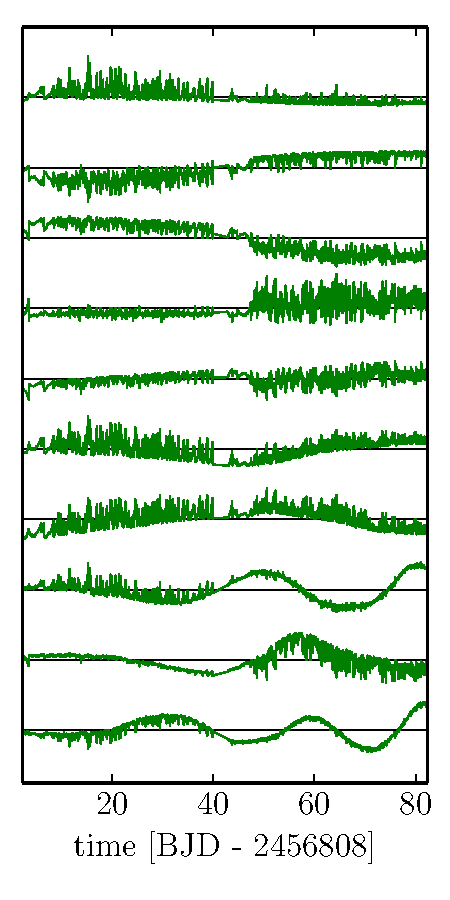
\includegraphics{figures/pca.pdf}
\end{center}
\caption{%
The top 10 eigen light curves (ELCs) generated by running principal component
analysis on all the aperture photometry from Campaign 1.
\figlabel{pca}}
\end{figure}

\begin{figure}[p]
\begin{center}
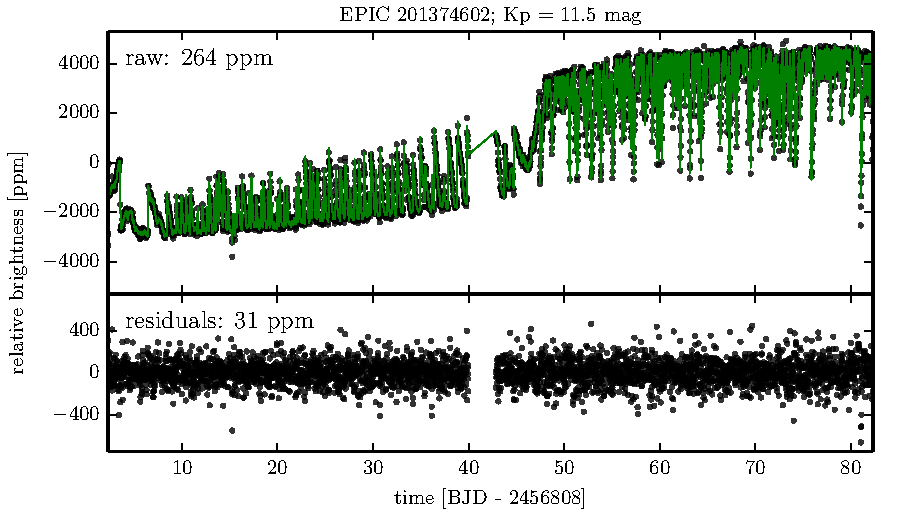
\includegraphics{figures/corr.pdf}
\end{center}
\caption{%
A demonstration of the ELC fit to the aperture photometry for EPIC 201374602.
\emph{Top:} The black points show the aperture photometry and the green line
is the maximum likelihood linear combination of ELCs.
The estimated 6-hour precision of the raw photometry is 264 ppm.
\emph{Bottom:} The points show the residuals of the data away from the ELC
prediction.
The 6-hour precision of this light curve is 31 ppm.
\figlabel{corr}}
\end{figure}

\begin{figure}[p]
\begin{center}
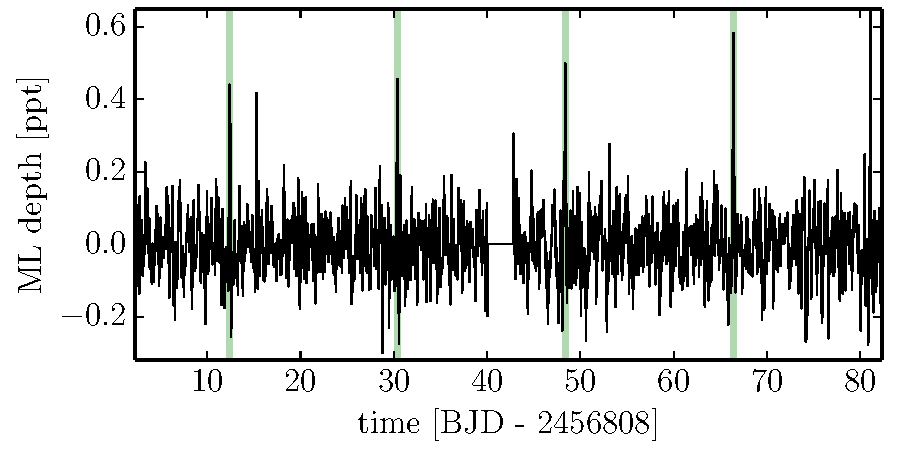
\includegraphics{figures/linear.pdf}
\end{center}
\caption{%
The estimated transit depth as a function of transit time as computed in a
linear search.
This light curve has an injected signal with transits at the times indicated
with green vertical lines.
\figlabel{linear}}
\end{figure}

\begin{figure}[p]
\begin{center}
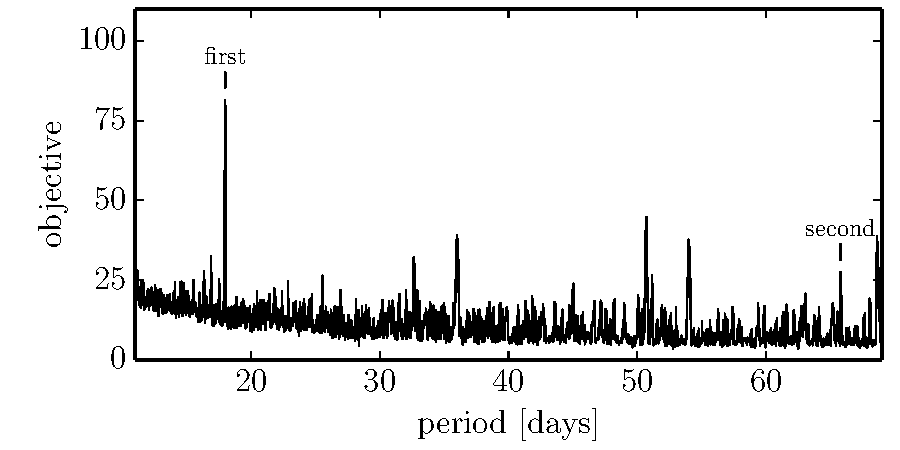
\includegraphics{figures/periodic.pdf}
\end{center}
\caption{%
The periodogram for the same signal as in \fig{linear}.
This plot was generated by the periodic search procedure.
The true period is indicated by the vertical green line.
\figlabel{periodic}}
\end{figure}

\begin{figure}[p]
\begin{center}
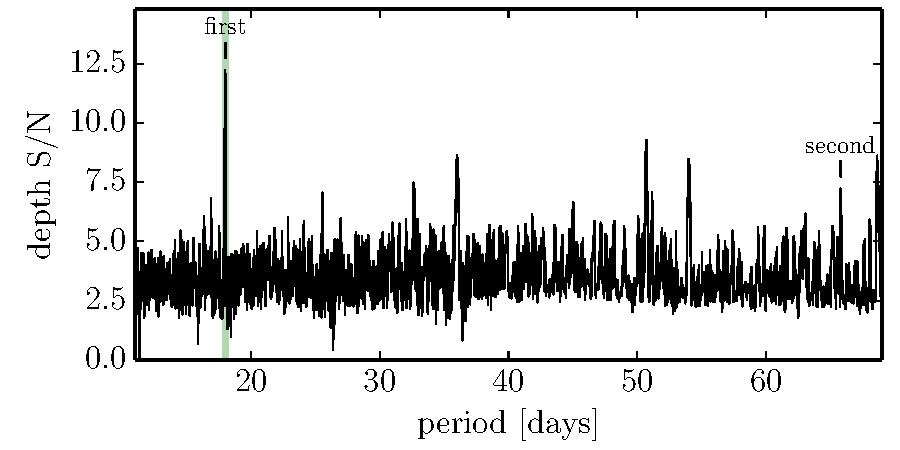
\includegraphics{figures/depth_s2n.pdf}
\end{center}
\caption{%
The signal-to-noise of the transit depth as a function of period for the same
signal as in \fig{periodic}.
The correct injected period is indicated by the vertical green line.
\figlabel{depth-s2n}}
\end{figure}

\begin{figure}[p]
\begin{center}
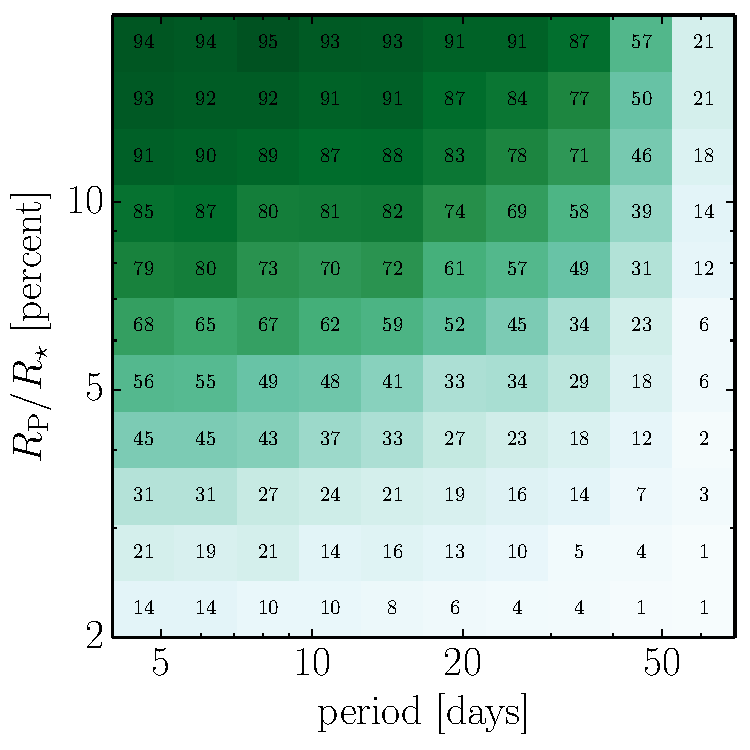
\includegraphics[width=\textwidth]{figures/completeness.pdf}
\end{center}
\caption{%
\figlabel{completeness}}
\end{figure}

\begin{table}[p]
\begin{center}
\small
\begin{tabular}{cccc}
\toprule
EPIC &  \period\ [days] & $t_0$ [BJD-2456808] & $R_\mathrm{P} / R_\star$ \\
\midrule
201208431 & $10.0040_{-0.0016}^{+0.0018}$ & $7.5216_{-0.0090}^{+0.0098}$ & $0.0349_{-0.0026}^{+0.0034}$ \\
201257461 & $50.2677_{-0.0074}^{+0.0083}$ & $20.3735_{-0.0098}^{+0.0147}$ & $0.0334_{-0.0017}^{+0.0054}$ \\
201280613 & $40.1205_{-0.0074}^{+0.0066}$ & $38.7724_{-0.0075}^{+0.0052}$ & $0.1508_{-0.0182}^{+0.0569}$ \\
201295312 & $5.6562_{-0.0007}^{+0.0007}$ & $3.7228_{-0.0091}^{+0.0086}$ & $0.0175_{-0.0009}^{+0.0020}$ \\
201338508 & $10.9328_{-0.0021}^{+0.0022}$ & $6.5967_{-0.0081}^{+0.0088}$ & $0.0339_{-0.0030}^{+0.0025}$ \\
201338508 & $5.7350_{-0.0006}^{+0.0006}$ & $0.8626_{-0.0055}^{+0.0054}$ & $0.0331_{-0.0023}^{+0.0025}$ \\
201367065 & $10.0542_{-0.0004}^{+0.0004}$ & $5.4186_{-0.0018}^{+0.0018}$ & $0.0354_{-0.0011}^{+0.0022}$ \\
201367065 & $24.6470_{-0.0016}^{+0.0014}$ & $4.2769_{-0.0029}^{+0.0030}$ & $0.0272_{-0.0013}^{+0.0016}$ \\
201384232 & $30.9375_{-0.0052}^{+0.0029}$ & $19.5035_{-0.0039}^{+0.0053}$ & $0.0260_{-0.0011}^{+0.0011}$ \\
201393098 & $28.6793_{-0.0116}^{+0.0105}$ & $16.6212_{-0.0177}^{+0.0305}$ & $0.0231_{-0.0020}^{+0.0028}$ \\
201403446 & $19.1535_{-0.0050}^{+0.0050}$ & $7.3437_{-0.0143}^{+0.0116}$ & $0.0154_{-0.0013}^{+0.0014}$ \\
201445392 & $10.3527_{-0.0011}^{+0.0011}$ & $5.6110_{-0.0051}^{+0.0047}$ & $0.0349_{-0.0025}^{+0.0045}$ \\
201445392 & $5.0644_{-0.0006}^{+0.0006}$ & $5.0690_{-0.0064}^{+0.0059}$ & $0.0274_{-0.0020}^{+0.0025}$ \\
201465501 & $18.4488_{-0.0015}^{+0.0015}$ & $14.6719_{-0.0032}^{+0.0035}$ & $0.0531_{-0.0039}^{+0.0061}$ \\
201505350 & $11.9069_{-0.0004}^{+0.0005}$ & $9.2764_{-0.0015}^{+0.0013}$ & $0.0446_{-0.0006}^{+0.0009}$ \\
201505350 & $7.9193_{-0.0001}^{+0.0001}$ & $5.3840_{-0.0008}^{+0.0006}$ & $0.0747_{-0.0013}^{+0.0016}$ \\
201546283 & $6.7713_{-0.0001}^{+0.0001}$ & $4.8453_{-0.0011}^{+0.0012}$ & $0.0481_{-0.0012}^{+0.0020}$ \\
201549860 & $5.6083_{-0.0006}^{+0.0005}$ & $4.1195_{-0.0047}^{+0.0045}$ & $0.0283_{-0.0023}^{+0.0041}$ \\
201555883 & $5.7966_{-0.0002}^{+0.0002}$ & $5.3173_{-0.0050}^{+0.0027}$ & $0.0604_{-0.0032}^{+0.0068}$ \\
201565013 & $8.6381_{-0.0002}^{+0.0003}$ & $3.4283_{-0.0015}^{+0.0016}$ & $0.1538_{-0.0243}^{+0.0355}$ \\
201569483 & $5.7969_{-0.0000}^{+0.0000}$ & $5.3130_{-0.0003}^{+0.0002}$ & $0.3587_{-0.0334}^{+0.0379}$ \\
201577035 & $19.3062_{-0.0013}^{+0.0013}$ & $11.5790_{-0.0027}^{+0.0025}$ & $0.0380_{-0.0012}^{+0.0023}$ \\
201593422 & $43.8753_{-0.0318}^{+0.0717}$ & $8.0383_{-0.0790}^{+0.0244}$ & $0.1366_{-0.0264}^{+0.0786}$ \\
201596316 & $39.8415_{-0.0155}^{+0.0136}$ & $21.8572_{-0.0101}^{+0.0120}$ & $0.0267_{-0.0022}^{+0.0034}$ \\
201613023 & $8.2818_{-0.0007}^{+0.0006}$ & $7.3752_{-0.0052}^{+0.0055}$ & $0.0205_{-0.0008}^{+0.0012}$ \\
201617985 & $7.2823_{-0.0008}^{+0.0007}$ & $4.6337_{-0.0050}^{+0.0050}$ & $0.0333_{-0.0032}^{+0.0072}$ \\
201629650 & $40.0492_{-0.0259}^{+0.0186}$ & $4.5363_{-0.0172}^{+0.0202}$ & $0.0241_{-0.0020}^{+0.0025}$ \\
201635569 & $8.3681_{-0.0002}^{+0.0002}$ & $3.4514_{-0.0014}^{+0.0015}$ & $0.0991_{-0.0078}^{+0.0120}$ \\
201649426 & $27.7704_{-0.0001}^{+0.0001}$ & $13.3476_{-0.0002}^{+0.0001}$ & $0.4365_{-0.0583}^{+0.0777}$ \\
201702477 & $40.7365_{-0.0025}^{+0.0026}$ & $3.5451_{-0.0025}^{+0.0026}$ & $0.0808_{-0.0114}^{+0.0043}$ \\
201736247 & $11.8106_{-0.0019}^{+0.0016}$ & $3.8483_{-0.0071}^{+0.0093}$ & $0.0347_{-0.0024}^{+0.0030}$ \\
201754305 & $19.0726_{-0.0049}^{+0.0048}$ & $1.4893_{-0.0133}^{+0.0128}$ & $0.0297_{-0.0030}^{+0.0042}$ \\
201754305 & $7.6202_{-0.0011}^{+0.0012}$ & $3.6813_{-0.0057}^{+0.0061}$ & $0.0281_{-0.0026}^{+0.0034}$ \\
201779067 & $27.2429_{-0.0001}^{+0.0001}$ & $12.2599_{-0.0003}^{+0.0002}$ & $0.2535_{-0.0259}^{+0.0369}$ \\
201828749 & $33.5093_{-0.0018}^{+0.0023}$ & $5.1554_{-0.0032}^{+0.0037}$ & $0.0267_{-0.0020}^{+0.0021}$ \\
201855371 & $17.9715_{-0.0017}^{+0.0015}$ & $9.9412_{-0.0038}^{+0.0033}$ & $0.0311_{-0.0017}^{+0.0030}$ \\
201912552 & $32.9410_{-0.0032}^{+0.0039}$ & $28.1834_{-0.0105}^{+0.0057}$ & $0.0513_{-0.0056}^{+0.0035}$ \\
201929294 & $5.0084_{-0.0001}^{+0.0001}$ & $4.5703_{-0.0012}^{+0.0022}$ & $0.1163_{-0.0014}^{+0.0011}$ \\
\bottomrule
\end{tabular}

\end{center}
\caption{%
Candidates
\tablabel{cand}}
\end{table}

\begin{table}[p]
\begin{center}
\begin{tabular}{cccc}
\toprule
EPIC & \period\ [days] & $t_0$ [BJD-2456808] & depth [ppt] \\
\midrule
201161715 & 59.81$^\mathrm{a}$ & 32.36 &  68.04 \\
201158453 &  7.07 &  5.46 &  72.75 \\
201160323 & 22.27 &  3.48 & 251.54 \\
201173390 & 17.00 &  8.40 &  31.34 \\
201333466 & 11.00 &  6.84 &  45.39 \\
201359834 & 40.11 & 30.66 &  11.92 \\
201368515 & 14.92 & 12.60 & 111.52 \\
201379113 & 42.41 & 14.24 & 210.28 \\
201382417 &  5.19 &  3.06 &  38.56 \\
201390608 &  9.81 &  4.58 &  82.85 \\
201408204 &  8.47 &  2.02 & 195.42 \\
201464977 & 15.89 &  1.50 &   8.18 \\
201530296 & 10.33 &  6.28 & 198.24 \\
201638314 &  5.43 &  4.30 &  49.66 \\
201648133 & 35.01 &  5.80 & 191.93 \\
201723461 & 22.73 & 22.14 & 262.30 \\
201763507 & 11.23 &  6.58 &   1.85 \\
201790675 & 33.83 & 29.10 & 352.43 \\
\bottomrule
\end{tabular}

\end{center}
\caption{%
Probable binaries.
\tablabel{eb}}
\end{table}

\end{document}
